%\documentclass{report}\begin{document}
\chapter{Origin of the Cube}
<<<<<<< .mine
\myTop{In this chapter the development and the problems with the patenting and legal issues regarding the cube are described. We will look at the patent to get a better understanding of the cubes made at the time. The purpose of this chapter is to give the reader a basic understanding of the \rubik{}. Furthermore we will describe the history behind \erno{} and how he got the idea for the \rubik{} to get a better understanding of the \rubik{}. 
=======
\myTop{In this chapter we will describe the history behind \erno{} and how he got the idea for the \rubik{} to get a better understanding of the \rubik{}. Furthermore we will look at the the development and the proble'matics with the patenting and legal issues regarding the cube are described. We will look at the patent to get a better understanding of the cubes made at the time. The purpose of this chapter is to give the reader a basic understanding of the \rubik{}.
>>>>>>> .r110
}
\section{Ern\"{o} Rubik}
\erno{} is the inventor behind the world famous \rubik{}. He was born in Budapest, Hungary in 1944, his father was flight engineer and his mother was poet. He graduated from the Technical University, Budapest as an architectural engineer after he graduated with a degree in architecture he stayed at the college to teach interior design.

That led to in \myDate{}{1}{1975} Rubik applied for a patent for his invention in Hungary There was made in first place to help his students. Two years later in 1977 he got the patent on the \mcube{}.
% Der er et spring fra Magic Cube til Rubiks Cube, som ikke beskrives
He became professor with full tenure in the 80s, he started Rubik Studio, which employs a dozen people to design furniture and toys. 
Since Rubik has produced several other toys, including Rubik's Snake, lately the studio began developing computer game. He also became the president of the Hungarian Engineering Academy in 1990. Same Year he created the International Rubik Foundation to support especially talented young engineers and industrial designers.
 
\section{Rubik's Cube(Magic Cube)}
In the 70s \erno{} was teaching Interior Design at Academy of Applied Arts and Crafts and he was trying to find a tool to help his students to understand three dimensional objects as result he made the \mcube in 1974 and obtained a Hungarian patent HU170062. 
% Det ovenover er allerede beskrevet i forrige section
Rubik got the idea for the cube when he wanted to make a three dimensional design with blocks that could move individually but many at the same time. Rubik initially tried  to make a cube that was held together with rubber bands but failed. Then he got the idea that the cubes had to hold each other in place, which resulted in a 3x3x3 cube that could \twist{} each \face{} individually. Rubik got the inspiration for the cube from the Magic Puzzle (see chapter \ref{chap:recreationalMathematics}).

Rubik described that some of the most important features behind the cube were that the parts of the cube stay together, which many other puzzles do not. He also pointed out that you can move several pieces at once. Also that it is three dimensional. 

In the end of 70s a Hungarian Businessman showed the Magic Cube at the Nuremberg toy fair and made it popular in Europe. The company Ideal Toy bought exclusive rights for the Magic Cube, but changed the name of the cube to \rubik{} within a year in order to get trademark protection.

At that time there were also two others applying for patent for products similar to the \rubik{}.  One of them was an American named Doctor Larry D. Nichols, and his cube was a 2x2x2 cube which was held together with magnets. The other one who applied for patent was a Japanese man named Terutoshi Ishige. He applied for patent a year after Rubik. Terutoshi Ishige's cube was almost identically to the \rubik{}.

Ideal Toy Company were bought by CBS Toy Company in 1982 and the trademark surpassed with it, but they sold the rights to Rubik's Cube to Seven Towns which is a Toy Company in Great Britain, they are still producing The Rubik's Cube today.
\section{The Nichols Cube Puzzle}
Dr. Larry D. Nichols studied chemistry at DePauw University in Greencastle, Indiana, before moving to Massachusetts to attend Harvard Graduate School. 
He is a lifelong puzzle enthusiast and inventor who  began developing a twist cube puzzle with six colored faces in 1957. It was made of eight smaller cubes assembled to a 2x2x2 cube. The eight cubes were held together by magnets.


\begin{figure}
	\centering
		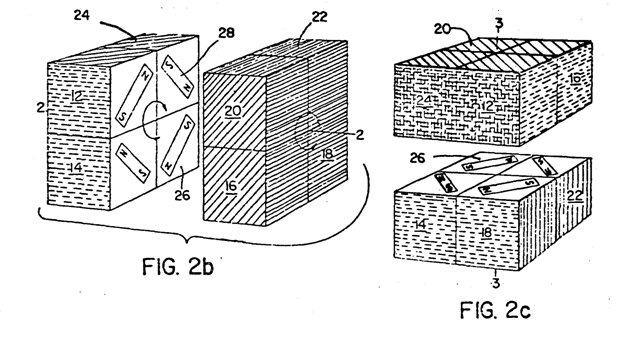
\includegraphics[scale=0.8]{input/pics/Nicholspatent2.png}
	\caption{\myCaption{Figure of Nichols Patent.}}
	\label{fig:Nicholspatent2}
\end{figure}


\textit{Give me a picture!} \\

On \myDate{11}{4}{1972} he was granted U.S. Patent 3,655,201 on behalf of Moleculon Research Corp. U.S. Patent 3,655,201 covered Nichols Cube and the possibility for making larger versions later. This was two years before \erno{} took out the patent for his \rubik{} in Hungary. 

In 1982 Moleculon Research corp.  Sued Ideal Toy Company that had the U.S. Patent 4,378,116 for \rubik{} because they believed that Ideal Toy Company violated their patent, but the U.S. District Court ruled in Ideal Toy Company favor. In 1986 the Court of Appeals ruled that the Pocket \rubik{} 2x2x2 was guilty of infringement but not the 3x3x3 \rubik{}.

\myTail{
In this chapter it has been described how \erno{} got the idea for the cube. We also stated that \erno{} was not the only one at that time, that came with the invention of cubes. \erno{}'s cube was special since the blocks hold each other together, which is different from the one Doctor Larry D. Nichols applied patent for which is hold together with magnets. 
}
%\end{document}